\pagebreak
\section{Verifica}
\label{sez:verifica}

La verifica è una fase cruciale del ciclo di vita del \textit{software}, finalizzata a garantire che il prodotto sviluppato soddisfi i requisiti specificati e sia privo di errori o difetti.\\
Questa attività si concentra sul controllo della correttezza, della completezza e della qualità del \textit{software}, sia a livello di codice che di comportamento.\\

\noindent La verifica può essere suddivisa in due approcci principali:

\begin{itemize}
\item \textbf{Analisi statica}:
È un processo che analizza il \textit{software} senza eseguirlo. \\
Si basa su tecniche di analisi statica, come le revisioni manuali del codice, l'uso di strumenti automatici per il controllo delle regole di codifica o per il \textit{linting} del codice. \\
Questo approccio consente di individuare errori, violazioni di standard, vulnerabilità e problemi di stile a livello di codice sorgente.  

\item \textbf{Analisi dinamica}:
Si basa sull’esecuzione del \textit{software} per testarne il comportamento in ambienti controllati o reali.\\
Questo approccio verifica che il sistema funzioni correttamente con \textit{input} specifici e che produca gli \textit{output} attesi. \\
Include attività come i \textit{test} unitari, \textit{test} di integrazione e \textit{test} di sistema.  
\end{itemize}

\noindent L’utilizzo combinato di analisi statica e dinamica è essenziale per garantire un livello elevato di qualità del \textit{software}. \\
Mentre l'analisi statica permette di affrontare i problemi a monte, l'analisi dinamica assicura che il sistema funzioni correttamente in condizioni operative. \\
Questo approccio integrato riduce al minimo il rischio di errori nel prodotto finale, migliorando l'affidabilità e la robustezza complessiva del \textit{software}.

\subsection{Analisi statica}
\label{subsec:analisi-statica}

Ho effettuato analisi statica per garantire che il codice sviluppato fosse conforme agli standard di qualità richiesti, riducendo la possibilità di errori e migliorandone la leggibilità e la manutenibilità.\\
Per questa attività ho utilizzato strumenti consolidati come \textit{Prettier} ed \textit{ESLint}, configurati per integrarsi con il flusso di lavoro del progetto.\\

\subsection{Analisi dinamica}
\label{subsec:analisi-dinamica}

Ho effettuato analisi dinamica per verificare il corretto funzionamento delle diverse componenti del sistema, con un particolare focus sul \gls{backend}, considerato il cuore del progetto, rispetto al \gls{frontend}, il cui \textit{testing} è stato affrontato solo in un secondo momento. \\
Le attività di \textit{testing} si sono concentrate prevalentemente sui \textit{test} unitari, con l'aggiunta di alcuni \textit{test} di performance per la generazione dei progetti.\\

\subsubsection{Testing del \gls{backend}}  

Ho sviluppato \textit{test} unitari per tutti i \textit{controller} ed i \textit{service}, assicurando la copertura di tutte le principali funzionalità del sistema.\\

\noindent I \textit{test} sono stati eseguiti durante tutto il ciclo di vita del \textit{software}, seguendo il modello a \textit{V} (visibile in {\hyperref[fig:v-model]{Figura 3.8}}), che prevede l’integrazione di attività di \textit{testing} in ogni fase di sviluppo.\\
    Man mano che venivano creati gli \textit{endpoint}, ho sviluppato i relativi \textit{test} per verificarne immediatamente la correttezza;

\noindent Questo approccio iterativo ha garantito che ogni componente fosse testata e verificata fin dalla sua creazione, riducendo al minimo la possibilità di accumulare errori e semplificando il \textit{debug} nelle fasi successive.\\

\begin{figure}[H]
    \centering
    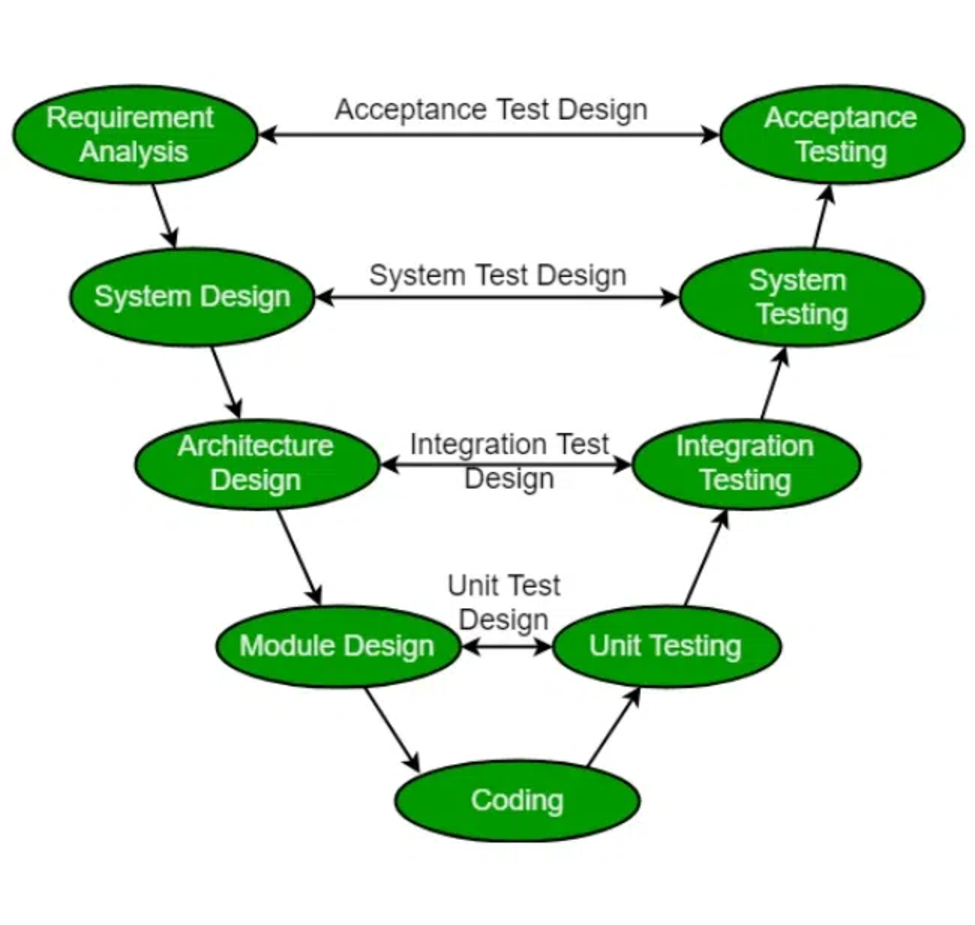
\includegraphics[scale=0.43]{v-model.png}
    \caption{Modello a V sviluppo \textit{software}}
    \label{fig:v-model}  
    \cite{site:v-model}
\end{figure}

\subsubsection{Test di performance}  
Ho effettuato alcuni \textit{test} di performance specifici per il \gls{backend}, con un focus particolare sulla generazione dei progetti.\\
Questi \textit{test} hanno permesso di misurare i tempi di risposta e verificare che il sistema fosse in grado di gestire la generazione di progetti in modo efficiente, anche in scenari di carico moderato.\\
